\documentclass{beamer}

\usetheme{Boadilla}
\usecolortheme{beaver}

\usepackage[utf8]{inputenc}
\usepackage[slovene,english]{babel}
\usepackage{graphicx}
\usepackage{amssymb}
\usepackage{amsmath}
\usepackage{array}
\usepackage{siunitx}
\usepackage{tikz}
\usetikzlibrary{positioning,shapes.geometric,arrows.meta,bending,positioning}
\usepackage{listings}

\tikzstyle{arrow} = [thick,->,>=stealth]

\newcommand{\PreserveBackslash}[1]{\let\temp=\\#1\let\\=\temp}
\newcolumntype{C}[1]{>{\PreserveBackslash\centering}p{#1}}
\newcolumntype{R}[1]{>{\PreserveBackslash\raggedleft}p{#1}}
\newcolumntype{L}[1]{>{\PreserveBackslash\raggedright}p{#1}}

\definecolor{codegreen}{rgb}{0,0.6,0}
\definecolor{codegray}{rgb}{0.5,0.5,0.5}
\definecolor{codepurple}{rgb}{0.58,0,0.82}
\definecolor{backcolour}{rgb}{0.95,0.95,0.92}
\definecolor{backcolour_func}{rgb}{0.90,0.90,0.90}

\lstset{
	language=C++,
	backgroundcolor=\color{backcolour},   
    commentstyle=\color{codegreen},
    keywordstyle=\color{magenta},
    numberstyle=\tiny\color{codegray},
    stringstyle=\color{codepurple},
    basicstyle=\fontsize{9}{9}\selectfont\ttfamily,
	breaklines=true,
	tabsize=2,
	numbers=left
}

\lstdefinestyle{func}{
	backgroundcolor=\color{white},
	basicstyle=\ttfamily\footnotesize,
	tabsize=4,
	numbers=none,
	frame=single
}

\title[Primerjava sistemskih klicev]{Primerjava sistemskih klicev \\operacijskih sistemov Linux in Windows}
\author[Miha Meglič]{Miha Meglič \\ \medskip Mentor: izr. prof. dr. Jurij Mihelič}
\institute[FRI]{Fakulteta za računalništvo in informatiko,\\Univerza v Ljubljani}
\date{12. september 2024}

\begin{document}

\frame{\titlepage}

\begin{frame}
	\frametitle{Operacijski sistemi}
	\begin{figure}
		\begin{center}
			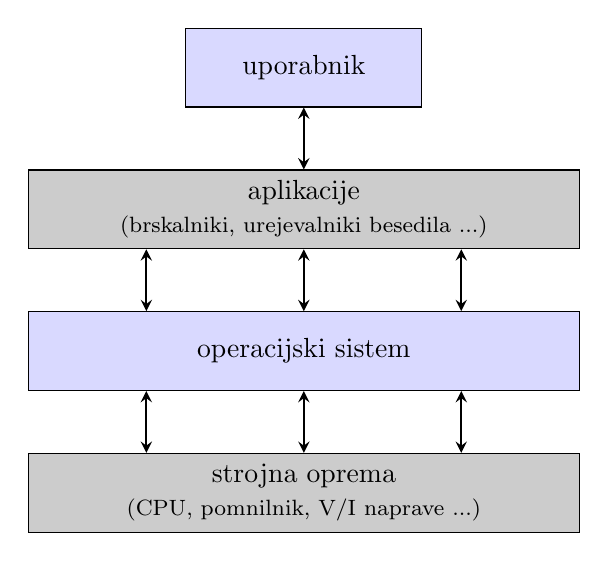
\begin{tikzpicture}[node distance=1.8cm]
				\tikzstyle{node} = [rectangle, draw=black, fill=blue!15!white, align=center, minimum height=1cm, minimum width=3cm];
				\node (user) [node] {uporabnik};
				\node (application) [node, minimum width=7cm, fill=gray!40!white, below of=user] {aplikacije\\\footnotesize{(brskalniki, urejevalniki besedila ...)}};
				\node (os) [node, minimum width=7cm, below of=application] {operacijski sistem};
				\node (hardware) [node, minimum width=7cm, fill=gray!40!white, below of=os] {strojna oprema\\\footnotesize{(CPU, pomnilnik, V/I naprave ...)}};
				\draw [thick,<->,>=stealth] (user) -- (application);
				\draw [thick,<->,>=stealth] ([xshift=2cm]application.south) -- ([xshift=2cm]os.north);
				\draw [thick,<->,>=stealth] (application) -- (os);
				\draw [thick,<->,>=stealth] ([xshift=-2cm]application.south) -- ([xshift=-2cm]os.north);
				\draw [thick,<->,>=stealth] ([xshift=2cm]os.south) -- ([xshift=2cm]hardware.north);
				\draw [thick,<->,>=stealth] (os) -- (hardware);
				\draw [thick,<->,>=stealth] ([xshift=-2cm]os.south) -- ([xshift=-2cm]hardware.north);
			\end{tikzpicture}
		\end{center}
	\end{figure}
\end{frame}

\begin{frame}
	\frametitle{Splošna primerjava sistemov}
	\begin{table}
		\begin{center}
			\begin{tabular}{ C{5cm}|C{5cm} }
				\textbf{Linux}             & \textbf{Windows}        \\
				\hline
				Linus Torvalds \& skupnost & Microsoft               \\
				samo jedro                 & poln operacijski sistem \\
				odprtokoden (GPL v2.0)     & zaprtokoden             \\
				POSIX, SUS                 & NT API                  \\
				glibc (GNU C knjižnica)   & Windows API             
			\end{tabular}
		\end{center}
	\end{table}
\end{frame}

\begin{frame}
	\frametitle{Programski vmesnik Linux}
	\begin{itemize}
		\item Dostopen preko GNU C knjižnice (glibc), ki poleg OS specifičnih vmesnikov implementira standarde ISO C11, POSIX.1-2008 in BSD
		      \begin{itemize}
		      	\item Izpostavlja nekaj sto funkcij (POSIX)
		      	\item Povezava funkcija--sistemski klic ni vedno ena proti ena
		      \end{itemize}
		\item Obstajajo tudi druge namenske knjižnice
	\end{itemize}
\end{frame}

\begin{frame}
	\frametitle{Programski vmesnik Windows}
	\begin{itemize}
		\item Implementiran v jedrnem programu (\textit{ntoskrnl.exe}) in uporabniški knjižnici (\textit{ntdll.dll})
		\item Dostopen preko Windows API
		      \begin{itemize}
		      	\item Izpostavlja več tisoč funkcij
		      	\item Dva interna kodiranja znakov -- Windows-1252 (``ANSI'') in UTF-16 (16-bitni Unicode)
		      \end{itemize}
	\end{itemize}
	\begin{table}
		\begin{center}
			\begin{tabular}{ l|l }
				Win32 API klic           & NT API klic                   \\
				\hline
				\texttt{CreateProcess}   & \texttt{NtCreateProcess}      \\
				\texttt{ReadFile}        & \texttt{NtReadFile}           \\
				\texttt{DeleteFile}      & \texttt{NtSetInformationFile} \\
				\texttt{DuplicateHandle} & \texttt{NtDuplicateObject}    \\
			\end{tabular}
		\end{center}
		\caption{Primeri Win32 API klicev in vezanih NT API klicev}
	\end{table}
\end{frame}

\begin{frame}
	\frametitle{Proces}
	\begin{itemize}
		\item Proces je program (strojna koda) v izvajanju
		\item Entiteta, ki zaseda sistemske vire
		\item Operacijski sistem v posebnem objektu beleži:
		      \begin{itemize}
		      	\item identifikator procesa (PID) in starša (PPID),
		      	\item stanje (življenjski cikel),
		      	\item programski števec,
		      	\item kazalec na sklad,
		      	\item pomnilniške dodelitve,
		      	\item tabelo odprtih objektov ...
		      \end{itemize}
	\end{itemize}
\end{frame}

\begin{frame}
	\frametitle{Proces v Linuxu}
	\begin{itemize}
		\item Procesi so organizirani v drevesno strukturo, kjer ima vsak proces svojega starša (razen \texttt{init})
		\item Procesi se identificirajo s PID
		\item Informacije procesa se hranijo v procesnem deskriptorju (\texttt{task\_struct})
		\item Niti so implementirane kot lahkotni procesi (\textit{angl. lightweight process})
		\item Niti se identificirajo s TID
	\end{itemize}
\end{frame}

\begin{frame}
	\frametitle{Proces v Windowsu}
	\begin{itemize}
		\item Funkcije večinoma uporabljajo ročice objektov (\textit{angl. handle}) namesto PID
		\item Ne strukturirano procesno drevo
		\item Informacije o procesu se hranijo v objektih \texttt{EPROCESS} in \texttt{KPROCESS}
		\item Niti so implementirane kot ločene entitete
		\item Informacije o niti se hranijo v objektih \texttt{ETHREAD} in \texttt{KTHREAD}
		\item Vsak proces ima vsaj eno nit, ki se imenuje glavna nit
	\end{itemize}
\end{frame}

\begin{frame}
	\frametitle{Ustvarjanje procesa v Linuxu}
	Linux implementira tri sistemske klice za ustvarjanje procesov:
	\begin{itemize}
		\item \texttt{fork} -- ustvari kopijo klicajočega procesa (Copy-on-Write)
		\item \texttt{vfork} -- ustvari kopijo klicajočega procesa, vendar se izvajanje nadaljuje v otroku
		\item \texttt{clone} -- ustvari nov proces z deljenimi viri (lahkotni proces) 
	\end{itemize}
																																																																		
	Vse tri so v jedru implementirane s funkcijo \texttt{do\_fork()}.
\end{frame}

\begin{frame}
	\frametitle{Ustvarjanje procesa v Windowsu}
	Novo ustvarjen proces se naloži iz programa in ni kopija starša.
	\begin{figure}
		\begin{center}
			\includegraphics[width=0.98\textwidth]{images/windows_createprocess_functions.png}
		\end{center}
		\caption{Funkcije za kreiranje procesa v Windowsu}
	\end{figure}
\end{frame}

\begin{frame}[fragile]
	\frametitle{Primerjava funkcij}
	Funkcije v Linuxu so tipično krajše in bolj jedrnate kot v Windowsu.
	\begin{lstlisting}[style=func]
 pid_t fork(void);
	\end{lstlisting}		
	\begin{lstlisting}[style=func]
 BOOL CreateProcessW(
	LPCWSTR               lpApplicationName,
	LPWSTR                lpCommandLine,
	LPSECURITY_ATTRIBUTES lpProcessAttributes,
	LPSECURITY_ATTRIBUTES lpThreadAttributes,
	BOOL                  bInheritHandles,
	DWORD                 dwCreationFlags,
	LPVOID                lpEnvironment,
	LPCWSTR               lpCurrentDirectory,
	LPSTARTUPINFOW        lpStartupInfo,
	LPPROCESS_INFORMATION lpProcessInformation
 );
	\end{lstlisting}
\end{frame}

\begin{frame}
	\frametitle{Kvantitativna primerjava -- Metodologija}
	\begin{itemize}
		\item Operacijska sistema:
		      \begin{itemize}
		      	\item Ubuntu Desktop 24.04 LTS
		      	\item Windows 10 Professional, verzija 22H2
		      \end{itemize}
		\item Programi za Linux so napisani v C in prevedeni z GCC, za Windows pa v C++ in prevedeni z MSVC.
		\item Za čas meritev je bil na Windowsu izklopljen Windows Defender.
	\end{itemize}
\end{frame}

\note{testtt}

\begin{frame}
	\frametitle{Primerjava izvajanja sistemskih klicev}
	Primerjamo sistemske klice za:
	\begin{table}
		\begin{center}
			\begin{tabular}{ l|c|c }
				                    & \textbf{Linux}  & \textbf{Windows}             \\
				\hline
				Ustvarjanje procesa & \texttt{fork}   & \texttt{CreateProcess}       \\
				Končanje procesa   & \texttt{kill}   & \texttt{TerminateProcess}    \\
				Ustvarjanje niti    & \texttt{clone}  & \texttt{CreateThread}        \\
				Končanje niti      & \texttt{kill}   & \texttt{TerminateThread}     \\
				Pridobivanje PID    & \texttt{getpid} & \texttt{GetCurrentProcessId} \\
			\end{tabular}
		\end{center}
	\end{table}
\end{frame}

\begin{frame}
	\frametitle{Primerjava izvajanja sistemskih klicev}
	Povprečni časi izvajanja sistemskih klicev:
	\begin{figure}
		\begin{center}
			\includegraphics[width=0.85\textwidth]{images/syscall_comparison_w5a.png}
		\end{center}
	\end{figure}
\end{frame}

\begin{frame}
	\frametitle{Primerjava programa}
	Scenarij:
	\begin{enumerate}
		\item Ustvari 2 grafična procesa -- na Linuxu bomo uporabili GNOME Text Editor, na Windowsu pa Notepad
		\item Izpiši PID obeh procesov
		\item Ustvari 10 niti, ki bodo neodvisno izračunale 40. število Fibonaccijevega zaporedja in zapisale rezultat v pomnilnik
		\item Izpiši TID vseh ustvarjenih niti
		\item Počakaj na zaključek niti
		\item Izpiši rezultat izračuna
		\item Prisilno končaj prej ustvarjena procesa
	\end{enumerate}
\end{frame}

\begin{frame}
	\frametitle{Primerjava programa}
	Povprečni časi izvajanja programa prevedenega brez optimizacij:
	\begin{figure}
		\begin{center}
			\includegraphics[width=0.7\textwidth]{images/program_comparison.png}
		\end{center}
	\end{figure}
\end{frame}

\begin{frame}
	\frametitle{Primerjava programa}
	Povprečni časi izvajanja programa prevedenega z optimizacijami:
	\begin{figure}
		\begin{center}
			\includegraphics[width=0.7\textwidth]{images/program_comparison_optimized.png}
		\end{center}
	\end{figure}
\end{frame}

\begin{frame}
	\frametitle{Ugotovitve}
	\begin{itemize}
		\item Funkcije Windows API so običajno bolj kompleksne.
		\item Linux je hitrejši pri ustvarjanju in končanju procesov in niti.
		\item Windows API opravi več dela v uporabniškem načinu.
		\item Delo z nitmi je veliko lažje v Windowsu.
		\item V Linuxu za kompleksnejše operacije običajno uporabljamo zunanje knjižnice.
	\end{itemize}
\end{frame}

\end{document}